\section{Theorie}
\label{sec:Theorie}

\subsection{Komplexe Widerstände}

Neben dem ohmschen Widerstand $R$, gibt es auch Spannungsabfälle bei Spulen der Induktivität $L$ und Kondensatoren der Kapazität $C$, 
sogennante \textit{Impedanzen}. Bei ohmschen Widerständen lässt sich der Spannungsabfall durch das \textit{Ohm'sche Gesetz} 

\begin{align*}
    U = R \cdot I    
\end{align*}

quantifizieren.

%Induktivitäten tun sich immer Verspäten
Da an Induktivitäten $L$ und Kapazitäten $C$ jedoch eine Phasenverschiebung zwischen Strom und Spannung auftritt, werden diese Widerstände
komplex dargestellt. Bei einem induktiven Widerstand wird der Wechselstrom durch eine Spule um $\SI{90}{\degree}$ gegenüber der 
Wechselspannung verzögert. Man definiert unter Berücksichtigung der Phasenverschiebung den induktiven Widerstand zu

\begin{align*}
    R_{\text{L}} = e^{-i\pi/2}\cdot\frac{U_0}{I_0} = i\cdot\omega L.
    %\label{eqn:indR}
\end{align*}

Wobei $i$ die imaginäre Einheit, $\omega$ die Kreisfrequenz der angelegten Wechselspannung und $L$ der Induktivität der Spule entspricht.
Bei einem kapazitiven Widerstand eilt der Strom der Spannung um $\SI{90}{\degree}$ voraus. Woraus sich der kapazitive Widerstand durch

\begin{align*}
    %\label{eqn:kapR}
    R_{\text{C}} = \frac UI = e^{-i\pi/2} \frac{U_0}{I_0} \\
    = \frac{1}{i\cdot\omega C}
\end{align*}

beschreiben lässt. Dabei entsprichen $i$ und $\omega$ analog zu oben der imaginären Einheit und der Kreisfrequenz der angelegten 
Wechselspannung und $C$ der Kapazität des Kondensators.
Somit hat die Impedanz $Z$ der drei in reihe geschalteten Widerstände die Beziehung

\begin{align}
    \label{eqn:impedanz}
    Z = R + i\cdot\omega L + \frac{1}{i\cdot\omega C}.
\end{align}


\subsection{Brückenschaltungen}
Brückenschaltungen basieren auf den Kirchhoff'schen Gesetzen, der Knoten- und Maschenregel, auf die hier nicht näher eingegangen werden soll.
In Brückenschaltungen werden Potentialdifferenzen zwischen zwei Punkten untersucht, die in Abhängigkeit zu ihren Widerstandsverhältnissen
stehen. Aus \autoref{fig:prinzipBruecke} lässt sich das Prinzip einer Brückenschaltung entnehmen.

\begin{figure}[H]
    \centering
    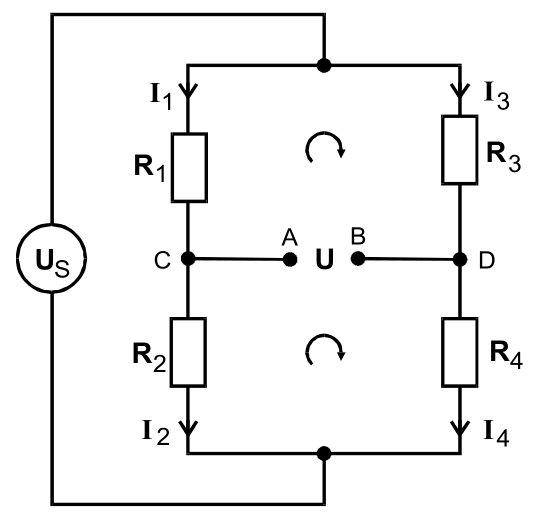
\includegraphics[width=0.75\textwidth]{dateien/PrinzipBrueckenschaltung.png}
    \caption{Schaltplan einesr grundlegenden Brückenschaltung \cite{anleitung}.}
    \label{fig:prinzipBruecke}
\end{figure}

Werden die Kirchhoff'schen Gesetze auf die Schaltung in \autoref{fig:prinzipBruecke} angewendet, so folgt ein Ausdruck
für die Brückenspannung in Abhängigkeit von den Schaltungsparametern

\begin{align*}
    U = \frac{R_2R_3 - R_1R_4}{(R_3+R_4)(R_1+R_2)} U_{\text{s}}  .
\end{align*}

%\nolinebreak
Der Ausdruck verschwindet, für den Fall einer abgeglichenen Brücke, unabhängig von der Höhe der Speisespannung, 
wenn der folgende Fall gegeben ist
\begin{align}
    \label{eqn:abgBr}
    R_1R_4=R_2R_3.
\end{align}


\subsection{Wheatstone'sche Messbrücke}
Bei einer Wheatsone'schen Messbrücke werden ausschließlich ohmsche Widerstände verwendet, um einen unbekannten Widerstand 
$R_{\text{x}}$ zu messen. Es wird der Widerstand $R_2$ festgehalten und ein Widerstandsverhältnis zwischen 
$R_3$ und $R_4$ wird mithilfe eines Potentiometers eingestellt. Somit ergibt sich die Gleichung einer abgeglichenen Brücke 
\ref{eqn:abgBr} im Fall einer Wheatstone'schen Messbrücke zu

\begin{align}
    R_{\text{x}} = R_2 \cdot \frac{R_3}{R_4}.
    \label{eqn:wheatstoneGleichung}
\end{align}

Aus \autoref{fig:wheatstone} ist das Schaltbild einer Wheatstone'schen Brücke abzulesen.

\begin{figure}[H]
    \centering
    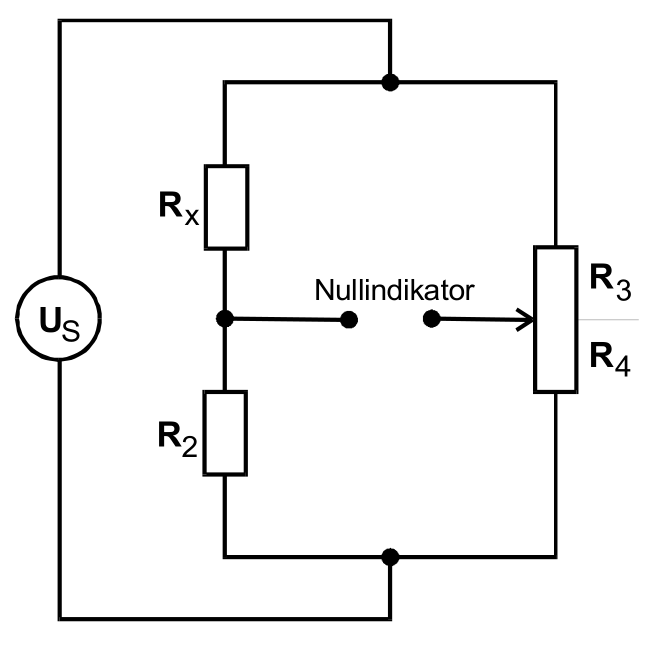
\includegraphics[width=0.75\textwidth]{dateien/wheatstoneBruecke.png}
    \caption{Schaltplan einer Wheatstone'schen Brücke \cite{anleitung}.}
    \label{fig:wheatstone}
\end{figure}


\subsection{Kapazitätsmessbrücke}
Da ein realer Kondensator durch dielektrische Verluste ein Teil seiner elektrischen Energie verliert, berücksichtigt
man diese Verluste dadurch, dass ein rein fiktiver Widerstand in Reihe mit dem Kondensator geschaltet wird.
Somit benötigt eine zur Messung einer unbekannten Kapazität $C_{\text{x}}$ einen weiteren Freiheitsgrad, um
die durch $R_{\text{x}}$ hervorgerufene Phasenverschiebung zu kompensieren. 
Aus \autoref{eqn:abgBr} folgt somit ein Zusammenhang für die Messung der unbekannten Größe $C_{\text{x}}$

\begin{align}
    C_{\text{x}} = C_2 \frac{R_4}{R_3}.
\end{align}

Eine solche Schaltung, wie sie auch in
\autoref{fig:schaltungb} abgebildet ist, wird \textit{Kapazitätsmessbrücke} genannt.

\begin{figure}[H]
    \centering
    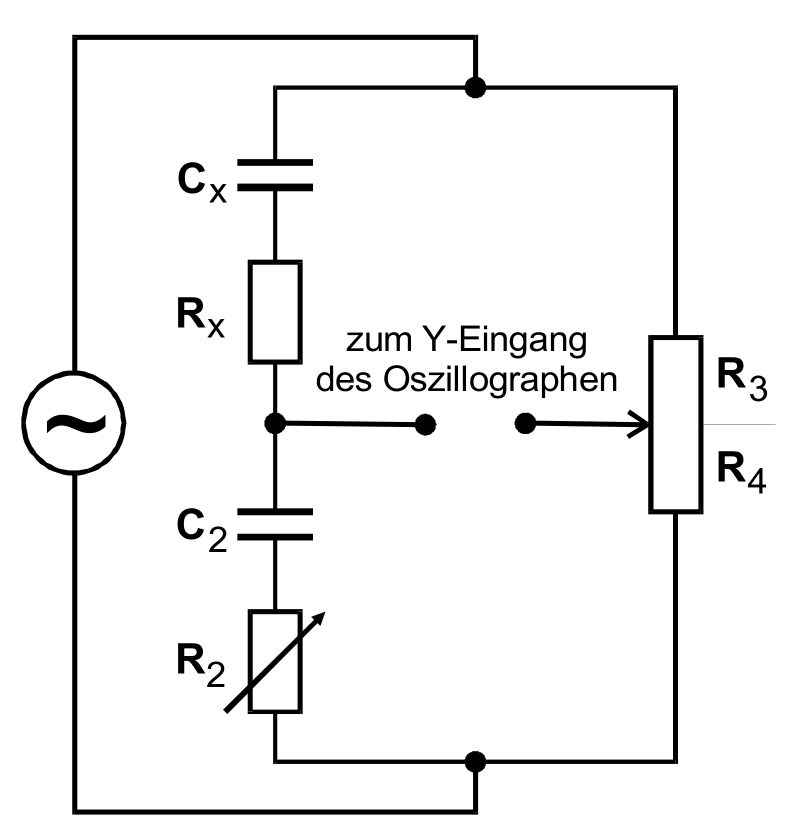
\includegraphics[width=0.75\textwidth]{dateien/aufgabeb).png}
    \caption{Schaltplan einer Kapazitätsmessbrücke \cite{anleitung}.}
    \label{fig:schaltungb}
\end{figure}

\subsection{Induktivitätsmessbrücke}

Eine Induktivitätsmessbrücke verhält sich analog zu einer Kapazitätsmessbrücke und folglich ergibt sich 
\autoref{eqn:abgBr} zu

\begin{align}
    L_{\text{x}} = L_2 \frac{R_4}{R_3}.
\end{align}

Ein Schaltbild für eine Induktivitätsmessbrücke ist \autoref{fig:schaltungc} zu entnehmen.

\begin{figure}[H]
    \centering
    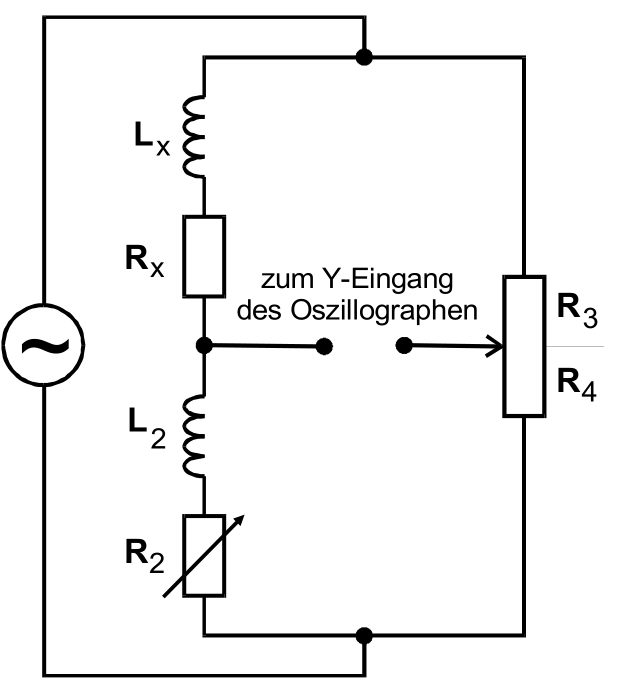
\includegraphics[width=0.75\textwidth]{dateien/aufgabec).png}
    \caption{Schaltplan einer Messbrücke für verlustbehaftete Induktivitäten \cite{anleitung}.}
    \label{fig:schaltungc}
\end{figure}

\subsection{Maxwell'sche Messbrücke}
Da der Wirkanteil im Brückenzweig einer Induktivitätsmessbrücke möglichst geringe Verluste besitzen sollte, dies aber
insbesondere bei niedrigen Frequenzen oft schwer zu realisieren ist, wird häufig auf eine Maxwell-Brücke ausgewichen, wie
sie auch in \autoref{fig:schaltungd} abgebildet ist.

\begin{figure}[H]
    \centering
    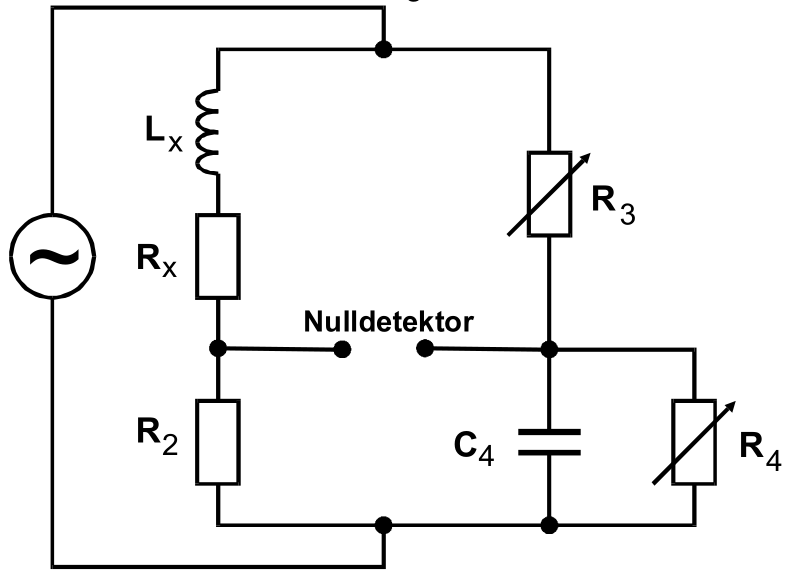
\includegraphics[width=0.75\textwidth]{dateien/aufgabed).png}
    \caption{Schaltplan einer Maxwell-Brücke \cite{anleitung}.}
    \label{fig:schaltungd}
\end{figure}

Da die Widerstandsoperatoren bei einer Maxwell-Brücke durch

\begin{align*}
    Z_{\text{x}} = R_{\text{x}} + i\cdot \omega L_{\text{x}}
\end{align*}

haben, folgt aus \autoref{eqn:abgBr} eine Relation für die unbekannte Induktivität $L_{\text{x}}$ zu

\begin{align}
    L_{\text{x}} = R_2R_3C_4.
\end{align}